\documentclass{beamer}

% packages [elementary]:
\usepackage{graphicx}
\usepackage[latin1]{inputenc}
\usepackage[T1]{fontenc}
\usepackage[english]{babel}
\usepackage{listings}
\usepackage{xcolor}
\usepackage{eso-pic}
\usepackage{mathrsfs}
\usepackage{url}
\usepackage{amssymb}
\usepackage{amsmath}
\usepackage{multirow}
\usepackage{hyperref}
\usepackage{caption}
\usepackage{siunitx}
\usepackage{booktabs}
\usepackage{hhline}

% packages [additional]
\usepackage{bbm}

% packages [ise-beamer]
\usepackage{cooltooltips}
\usepackage{colordef}
\usepackage{beamerdefs}
\usepackage{lvblisting}

% "logobig" and "logosmall" pictures [internal names, do not modify] 
\pgfdeclareimage[height=2cm]{logobig}{hulogo}
% individual logo: change the file name to "logo" [lower right corner]
\pgfdeclareimage[height=0.7cm]{logosmall}{OilRig}

% titlle page [layout]:
% scaling of the headline on title page
\renewcommand{\titlescale}{1.0}
% title page with two columns [following two values: determine the percentage each one should get]
\renewcommand{\titlescale}{1.0}
\renewcommand{\leftcol}{0.6}

% document title & title abbreviation [footer]
\title[SPL - US Energy Sector Analysis]{Statistical Programming Languages (SPL): United States Oil Company Analysis}
% authors:
\authora{Marcus Goossens} % a-c
\authorb{Tim Halbmann}
\authorc{Antton Haramboure
\\Fabian Salger}

% links [for display on title page]
\def\linka{}
\def\linkb{}
\def\linkc{}

% institute:
\institute{Group-project presentation at the \\
Ladislaus von Bortkiewicz Chair of Statistics \\
Humboldt--Universit�t zu Berlin \\}

\newcommand{\qletz}{\raisebox{-1pt}{
\includegraphics[scale=0.05]{qletlogo}}}

% pdf file starts in full screen mode [tool for presentation day]
\hypersetup{pdfpagemode=FullScreen}

%%%%%%%%%%%%%%%%%%%%%%%%%%%%%%%%%%%%%%%%%%%%%%%%%%%%%%%%%%%%%%%%%%%%%%%%%%%%%%%%%%%%%%%%%%%%%%%%%%%%%%%%%%%%%%%%%%%%%%%%
%%%%%%%%%%%%%%%%%%%%%%%%%%%%%%%%%%%%%%%%%%%%%%%%%%%%%%%%%%%%%%%%%%%%%%%%%%%%%%%%%%%%%%%%%%%%%%%%%%%%%%%%%%%%%%%%%%%%%%%%

\begin{document}

% title slide, beamerdefs.sty [layout]
\frame[plain]{
\titlepage
}

%%%%%%%%%%%%%%%%%%%%%%%%%%%%%%%%%%%%%%%%%%%%%%%%%%%%%%%%%%%%%%%%%%%%%%%%%%%%%%%%%%%%%%%%%%%%%%%%%%%%%%%%%%%%%%%%%%%%%%%%
% outline w/o slide number
\useheadtemplate{
	\raisebox{-0.75cm}{\parbox{\textwidth}{
			\footnotesize{\color{isegray}
				\insertsection\ \leavevmode\leaders\hrule height3.2pt depth-2.8pt\hfill\kern0pt\ }}}}

\frame{
\frametitle{Outline}
\begin{enumerate}
\item Introduction
\item Dataset Transformations
\item Exploratory Analysis: Plots \& Graphics
\item Panel Data Regression \& Results
\item Applications
\begin{itemize}
\item Firm Types
\item Further Applications
\end{itemize} 
\item Literature
\end{enumerate}
}

% use slide number after outline
\useheadtemplate{
	\raisebox{-0.75cm}{\parbox{\textwidth}{
			\footnotesize{\color{isegray}
				\insertsection\ \leavevmode\leaders\hrule height3.2pt depth-2.8pt\hfill\kern0pt\ \thesection-\thepage}}}}
\setcounter{section}{0}

%%%%%%%%%%%%%%%%%%%%%%%%%%%%%%%%%%%%%%%%%%%%%%%%%%%%%%%%%%%%%%%%%%%%%%%%%%%%%%%%%%%%%%%%%%%%%%%%%%%%%%%%%%%%%%%%%%%%%%%%
\section{Introduction}
%%%%%%%%%%%%%%%%%%%%%%%%%%%%%%%%%%%%%%%%%%%%%%%%%%%%%%%%%%%%%%%%%%%%%%%%%%%%%%%%%%%%%%%%%%%%%%%%%%%%%%%%%%%%%%%%%%%%%%%%

\frame[containsverbatim]{
\vspace{-4.5cm}
\frametitle{Stock Returns: US Oil-Companies}
\begin{figure}[ht]
\begin{center}

\includegraphics[scale=0.5]{All_Stocks_Plot}
\end{center}
\end{figure}
\vspace{-0.5cm}
}

\frame{
\frametitle{Companies in the Sample}
\begin{table}[ht]
\begin{tabular}{l |c}
\hhline{==}
%\hline
& \\[-0.4cm]
\multicolumn{1}{c|}{Company} & \multicolumn{1}{c}{Remark}  \\
\hline
& \\[-0.4cm]
Chevron &  \\ 
  Exxon Mobil &  \\ 
  Apache &  \\ 
  Hess Corp &  \\ 
  Occidental Petrolium &  \\ 
  Murphy Oil &  \\
  CPEnergy & ($\ast$) \\
  PGE Corp & ($\ast$) \\
  Williams Cos, Inc. & ($\ast\ast$) \\
   \hline
   \hline
\multicolumn{2}{c}{\footnotesize note: ($\ast$) utility sector; ($\ast\ast$) EDA-Case} \\
\end{tabular}
\setbeamerfont{caption}{size=\small} 
\caption{Sample Companies} 
  \label{} 
\end{table}
}

\frame{
\frametitle{Model Environment}
\begin{itemize}
\item Bianconi/Yoshino (2014), Boyer/Filion (2006)
    \begin{itemize}
    \item framework adaptation
    \end{itemize}
\item Theory: Capital Asset Pricing Model (CAPM)
    \begin{itemize}
    \item assumptions include frictionless (financial) markets \& symmetric information
    \end{itemize}
\item Model: Panel Data Regression
\item Data source: Bloomberg
\end{itemize}
}

%%%%%%%%%%%%%%%%%%%%%%%%%%%%%%%%%%%%%%%%%%%%%%%%%%%%%%%%%%%%%%%%%%%%%%%%%%%%%%%%%%%%%%%%%%%%%%%%%%%%%%%%%%%%%%%%%%%%%%%%
\section{Transformations}
%%%%%%%%%%%%%%%%%%%%%%%%%%%%%%%%%%%%%%%%%%%%%%%%%%%%%%%%%%%%%%%%%%%%%%%%%%%%%%%%%%%%%%%%%%%%%%%%%%%%%%%%%%%%%%%%%%%%%%%%

\frame{
\frametitle{Data Source [raw]: Bloomberg}
\begin{itemize}
\item Data source [raw]: Bloomberg
\item Dataset issues addressed:
   \begin{itemize}
   \item class of data variable-dependent (e.g. date, returns)
   \item common data vary over time
   \item specific data vary over both time \& company
   \end{itemize}
\end{itemize}
}

\frame{
\frametitle{Transformations applied on Variables}
\vspace{-1cm}
\begin{table}[ht]
\setbeamerfont{caption}{size=\small} 
\caption{Variables by Transformation Mode} 
  \label{} 
\centering
\begin{tabular}{l|l|ll}
\hline
\hline
\multicolumn{1}{l|}{log return} & \multicolumn{1}{l|}{z-score} & \multicolumn{1}{c}{log} \\
\hline
Stock & NI & A.MCAP\\ 
 Oil &BVE.MCAP &  D.MCAP\\ 
 Gas& & \\ 
 Market(*)& &\\ 
 EX(**)& & \\ 
   \hline
   \hline
\multicolumn{4}{l}{\footnotesize (*): Dow Jones Industrial Average (DJI)} \\
\multicolumn{4}{l}{\footnotesize (**): USD wrt. EUR, GBP, ...}
\end{tabular}
\end{table}
}

%%%%%%%%%%%%%%%%%%%%%%%%%%%%%%%%%%%%%%%%%%%%%%%%%%%%%%%%%%%%%%%%%%%%%%%%%%%%%%%%%%%%%%%%%%%%%%%%%%%%%%%%%%%%%%%%%%%%%%%%
\section{Exploratory Analysis}
%%%%%%%%%%%%%%%%%%%%%%%%%%%%%%%%%%%%%%%%%%%%%%%%%%%%%%%%%%%%%%%%%%%%%%%%%%%%%%%%%%%%%%%%%%%%%%%%%%%%%%%%%%%%%%%%%%%%%%%%

\frame[containsverbatim]{
\frametitle{Distress Case, Firm 9: Williams}
\begin{table}[ht]
\small
\centering
\begin{tabular}{l|SSSS}
  \hline
\hline
\multicolumn{1}{c|}{Firm 9: \emph{Williams}} & \multicolumn{1}{c}{$\mu$} & \multicolumn{1}{c}{$\sigma$} & \multicolumn{1}{c}{$\mbox{Min}$} & \multicolumn{1}{c}{$\mbox{Max}$}  \\ 
  \hline
  Stock & 23.39 & 12.05 & 1.85 & 58.21 \\ 
  A.MCAP & 3.01 & 4.63 & 0.80 & 30.73 \\ 
  BVE.MCAP & 0.66 & 0.70 & 0.13 & 4.96 \\ 
  D.MCAP [\%] & 151.40 & 58.77 & 85.06 & 337.28 \\ 
  NI & 68.53 & 350.20 & -1263.00 & 1678.00 \\ 
   \hline
\hline
\end{tabular}
\caption{Exploratory data analysis - event detection} 
\end{table}
\begin{lstlisting}
# Summary statistics of company-specific variables
SumSpecF = describeBy(data[,2:7], group = "Company", 
                      mat = TRUE, digits = 2,
                      trim = 0, type = 1)
\end{lstlisting}
\begin{center}
\begin{small}
\vspace{-0.1cm}
Quantlet 2 - EDA: Lines 45 to 48 \href{https://github.com/Fabian-HC/SPL-OilUS/blob/master/EDA_PanDat/EDA_PanDat.R}{\protect \qletz}\\[0.5cm]
\end{small}
\end{center}
}

\frame[containsverbatim]{
\frametitle{Distress Case, Firm 9: Williams}
\begin{itemize}
\item Williams close to bankruptcy around 2002-2003
\end{itemize}
\begin{figure}[ht]
\vspace{-1.8cm}
\begin{center}
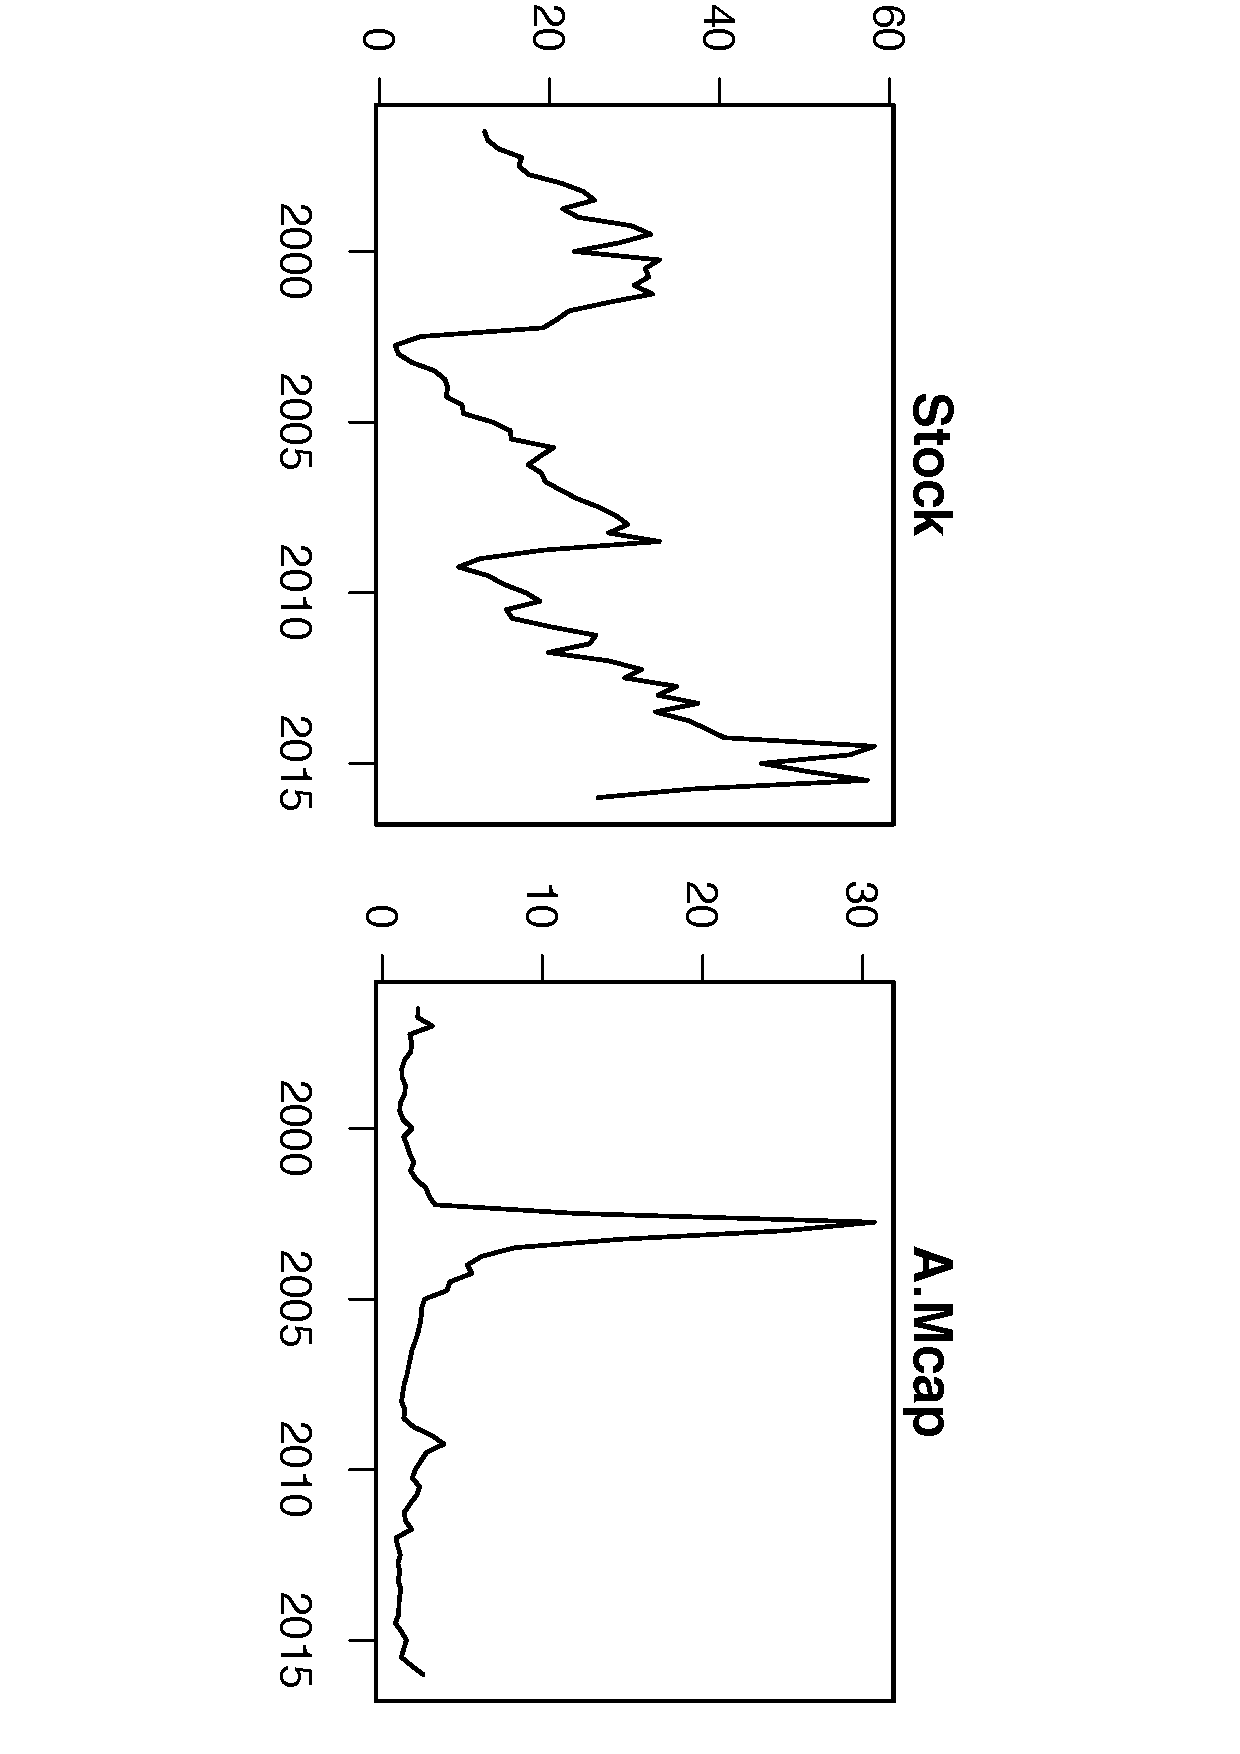
\includegraphics[scale=0.35,angle=90]{C9_WilliamsPresentation}
\end{center}
\vspace{-2cm}
\caption{Financial Distress Case of C9: Williams}
\end{figure}
}

%%%%%%%%%%%%%%%%%%%%%%%%%%%%%%%%%%%%%%%%%%%%%%%%%%%%%%%%%%%%%%%%%%%%%%%%%%%%%%%%%%%%%%%%%%%%%%%%%%%%%%%%%%%%%%%%%%%%%%%%
\section{Regression \& Results}
%%%%%%%%%%%%%%%%%%%%%%%%%%%%%%%%%%%%%%%%%%%%%%%%%%%%%%%%%%%%%%%%%%%%%%%%%%%%%%%%%%%%%%%%%%%%%%%%%%%%%%%%%%%%%%%%%%%%%%%%

\frame{
\frametitle{Panel Regression: Main Results}
\begin{table}[ht]
\setbeamerfont{caption}{size=\small} 
\caption{Panel Data Regression: Random Effects Model} 
  \label{} 
\centering
\begin{tabular}{l |S l}
\hline
\hline
\multicolumn{1}{c|}{Variable} & \multicolumn{1}{c}{$\beta$} & \multicolumn{1}{c}{} \\
\hline
(Intercept) & 0.01 &  \\ 
  NI & 0.01 & ** \\ 
  BVE.MCAP & -0.04 & *** \\ 
  D.MCAP & 0.00 &  \\ 
  Oil & 0.26 & *** \\ 
  Gas & 0.07 & *** \\ 
  Market & 0.72 & *** \\ 
   \hline
   \hline
\multicolumn{3}{c}{\footnotesize note: $^{*}$p$<$0.1; $^{**}$p$<$0.05; $^{***}$p$<$0.01} \\
\multicolumn{3}{l}{\footnotesize adj. R$^{2}$ = 0.40}
\end{tabular}
\end{table}
}

\frame[containsverbatim]{
\frametitle{Random Effects Model: Regression Output}
\begin{center}
$R_{it} = \alpha + \beta_{1}NI_{it} + [...] + \beta_{6} Market_{it} + \mu_i + \epsilon_{it}$
\end{center}
\begin{itemize}
\item Oil and gas price have robust positive effect on stock prices
    \begin{itemize}
    \item higher prices indicate presence of a profitable environment for oil companies
    \end{itemize}
\item Exposure of stock prices to the U.S. DJI market premium is robustly priced and positive
     \begin{itemize}
     \item energy consumption is related to overall economic situation
     \end{itemize}
\item Non-systematic risk factors are robustly priced
\end{itemize}
}

%%%%%%%%%%%%%%%%%%%%%%%%%%%%%%%%%%%%%%%%%%%%%%%%%%%%%%%%%%%%%%%%%%%%%%%%%%%%%%%%%%%%%%%%%%%%%%%%%%%%%%%%%%%%%%%%%%%%%%%%
\section{Applications}
%%%%%%%%%%%%%%%%%%%%%%%%%%%%%%%%%%%%%%%%%%%%%%%%%%%%%%%%%%%%%%%%%%%%%%%%%%%%%%%%%%%%%%%%%%%%%%%%%%%%%%%%%%%%%%%%%%%%%%%%
\subsection{Firm Type}

\frame[containsverbatim]{
\frametitle{Application Result: By Company Type}
\begin{itemize}
\item A comparison of the impact of common factors on:
\begin{itemize}
\item Oil-/ Gas-producing
\item Electricity-producing
\end{itemize}
\end{itemize}
\begin{equation}
R_{it} = \beta _{0}^{oil}+ O'_{it}\beta _{1}^{oil}+ B'_{it}\beta _{2}^{oil}+ M'_{it}\beta _{3}^{oil} +E'_{it}\beta _{4}^{oil}+\varepsilon _{it}
\end{equation}
\begin{equation}
R_{it} = \beta _{0}^{elec}+ O'_{it}\beta _{1}^{elec}+ B'_{it}\beta _{2}^{elec}+ M'_{it}\beta _{3}^{elec} +E'_{it}\beta _{4}^{elec}+\varepsilon _{it}
\end{equation}
\begin{small}
\begin{equation}
R_{it} = \beta _{0}+ O'_{it}\beta _{1}+ [...] +D^{elec}\beta _{5}+ D^{elec}O'_{it}\beta _{6}+ [...] +D^{elec}E'_{it}\beta _{9}+\varepsilon _{it}
\end{equation}
\end{small}
}

\frame[containsverbatim]{
\frametitle{Random Effects Models: Company Types}
\begin{itemize}
\item $\beta^{(1)}$: Oil-based Model
\item $\beta^{(2)}$: Electricity-based Model
\end{itemize}
\begin{table}[ht]
  \caption{Random Effect Model depending on Company type} 
  \label{} 
\centering
\begin{tabular}{l |S lS l}
  \hline
  \hline
\multicolumn{1}{c|}{Variable} & \multicolumn{1}{c}{$\beta^{(1)}$} & \multicolumn{1}{c}{} & \multicolumn{1}{c}{$\beta^{(2)}$} & \multicolumn{1}{c}{} \\
  \hline
(Intercept) & 0.02 & *** & 0.01 &  \\ 
  Oil & 0.31 & *** & -0.10 & * \\ 
  Gas & 0.07 & *** & 0.10 & ** \\ 
  Market & 0.68 & *** & 0.60 & *** \\ 
  EURUSD & 0.03 &  & -0.02 &  \\ 
   \hline
   \hline
\multicolumn{1}{c}{} & \multicolumn{2}{c}{\footnotesize adj. R$^{2}$ = 0.32 } & \multicolumn{2}{c}{\footnotesize adj. R$^{2}$ = 0.14 } \\
\multicolumn{5}{c}{\footnotesize note: $^{*}$p$<$0.1; $^{**}$p$<$0.05; $^{***}$p$<$0.01}
\end{tabular}
\end{table}
}

\subsection{Further Applications}

\frame[containsverbatim]{
\frametitle{Further Applications}
\begin{itemize}
\item Seasonality Effects
\bigskip
\item Impact of the financial crisis around 2008
\begin{itemize}
\item subsample and dummy test performed
\end{itemize}
\end{itemize}
}

%%%%%%%%%%%%%%%%%%%%%%%%%%%%%%%%%%%%%%%%%%%%%%%%%%%%%%%%%%%%%%%%%%%%%%%%%%%%%%%%%%%%%%%%%%%%%%%%%%%%%%%%%%%%%%%%%%%%%%%%
\section{Literature}
%%%%%%%%%%%%%%%%%%%%%%%%%%%%%%%%%%%%%%%%%%%%%%%%%%%%%%%%%%%%%%%%%%%%%%%%%%%%%%%%%%%%%%%%%%%%%%%%%%%%%%%%%%%%%%%%%%%%%%%%

\frame{
\frametitle{Bibliography}
\begin{thebibliography}{aaaaaaaaaaaaaaaaa}
\beamertemplatearticlebibitems
\bibitem{Bianconia/Yoshinob:2014}
Marcelo Bianconi, Joe A. Yoshino
\newblock{\em Risk factors and value at risk in publicly traded companies of the nonrenewable energy sector}
\newblock available on \href{http://www.sciencedirect.com/science/article/pii/S0140988314001510}{www.sciencedirect.com}, 2014
\beamertemplatearticlebibitems
\bibitem{Boyer/Filion:2007}
M. Martin Boyer, Didier Filion
\newblock{\em Common and fundamental factors in stock returns of Canadian oil and gas companies}
\newblock available on \href{http://www.sciencedirect.com/science/article/pii/S0140988305001167}{www.sciencedirect.com}, 2007
\end{thebibliography}
}

\end{document}
